\documentclass[12pt,twoside]{article}
%--------------------------------------------------------------------
\usepackage{graphicx,color,fancyhdr,amssymb,amsmath,wasysym}
%\usepackage{graphtex}
\usepackage[T1]{fontenc}
\usepackage[left=1.0in,right=0.75in,top=1.25in,bottom=1.5in]{geometry}
\geometry{papersize={8.5in,11in}}
\def\R{\mathbb{R}}
%--------------------------------------------------------------------
\newtheorem{exercise}{\bf Exercises}[section]
\newtheorem{theorem}{\bf Theorem}[section]
\newtheorem{definition}[theorem]{\bf Definition}
\newtheorem{example}[theorem]{\bf Example}
\newtheorem{remark}[theorem]{\bf Remark}
%--------------------------------------------------------------------
\pagestyle{fancy}
\fancyhead{}
\fancyfoot{}
\fancyhead[LE]{\sffamily \thepage}
\fancyhead[RE]{\sffamily\leftmark}
\fancyhead[RO]{\sffamily \thepage}
\fancyhead[LO]{\sffamily C.P.G}
\fancyfoot[CO]{\sffamily Mat061 Calculus II}
\fancyfoot[CE]{\sffamily Polar Coordinate System}
\renewcommand{\headrulewidth}{0mm}
%--------------------------------------------------------------------
\begin{document}
%--------------------------------------------------------------------
\title{The Polar Coordinate System\footnote{A topic in Mat061 at the Department of Mathematics and Statistics, MSU-IIT}}
\author{{\sffamily Charlene P. Garridos}\\
Undergraduate Student\\Bachelor of Science in Statistics}
\date{\today}
%--------------------------------------------------------------------
\maketitle
\tableofcontents
%--------------------------------------------------------------------
\begin{abstract}
So far, you have been representing graphs as collections of points (x,y) on the rectangular coordinate system. The corresponding equations for these graphs have been in either rectangular or parametric form. In this section you will study a coordinate system called the \textbf{polar coordinate system}. Students are expected to understand the polar coordinate system, polar graphs and rewrite the rectangular coordinates and equations in polar form and vice versa.
\end{abstract}
%--------------------------------------------------------------------
\section{The Polar Coordinate System}

\subsection{The Rectangular and Polar Coordinate Systems}

To form the polar coordinate system in the plane, fix a point \emph O, called the \textbf{pole} (or \textbf{origin}), and construct from \emph O an initial ray called the \textbf{polar axis}, as shown in Figure 10.36. Then each point \emph P in the plane can be assigned \textbf {polar coordinates} $ (r, \theta)$, as follows.

\begin{figure}[h]
\centering
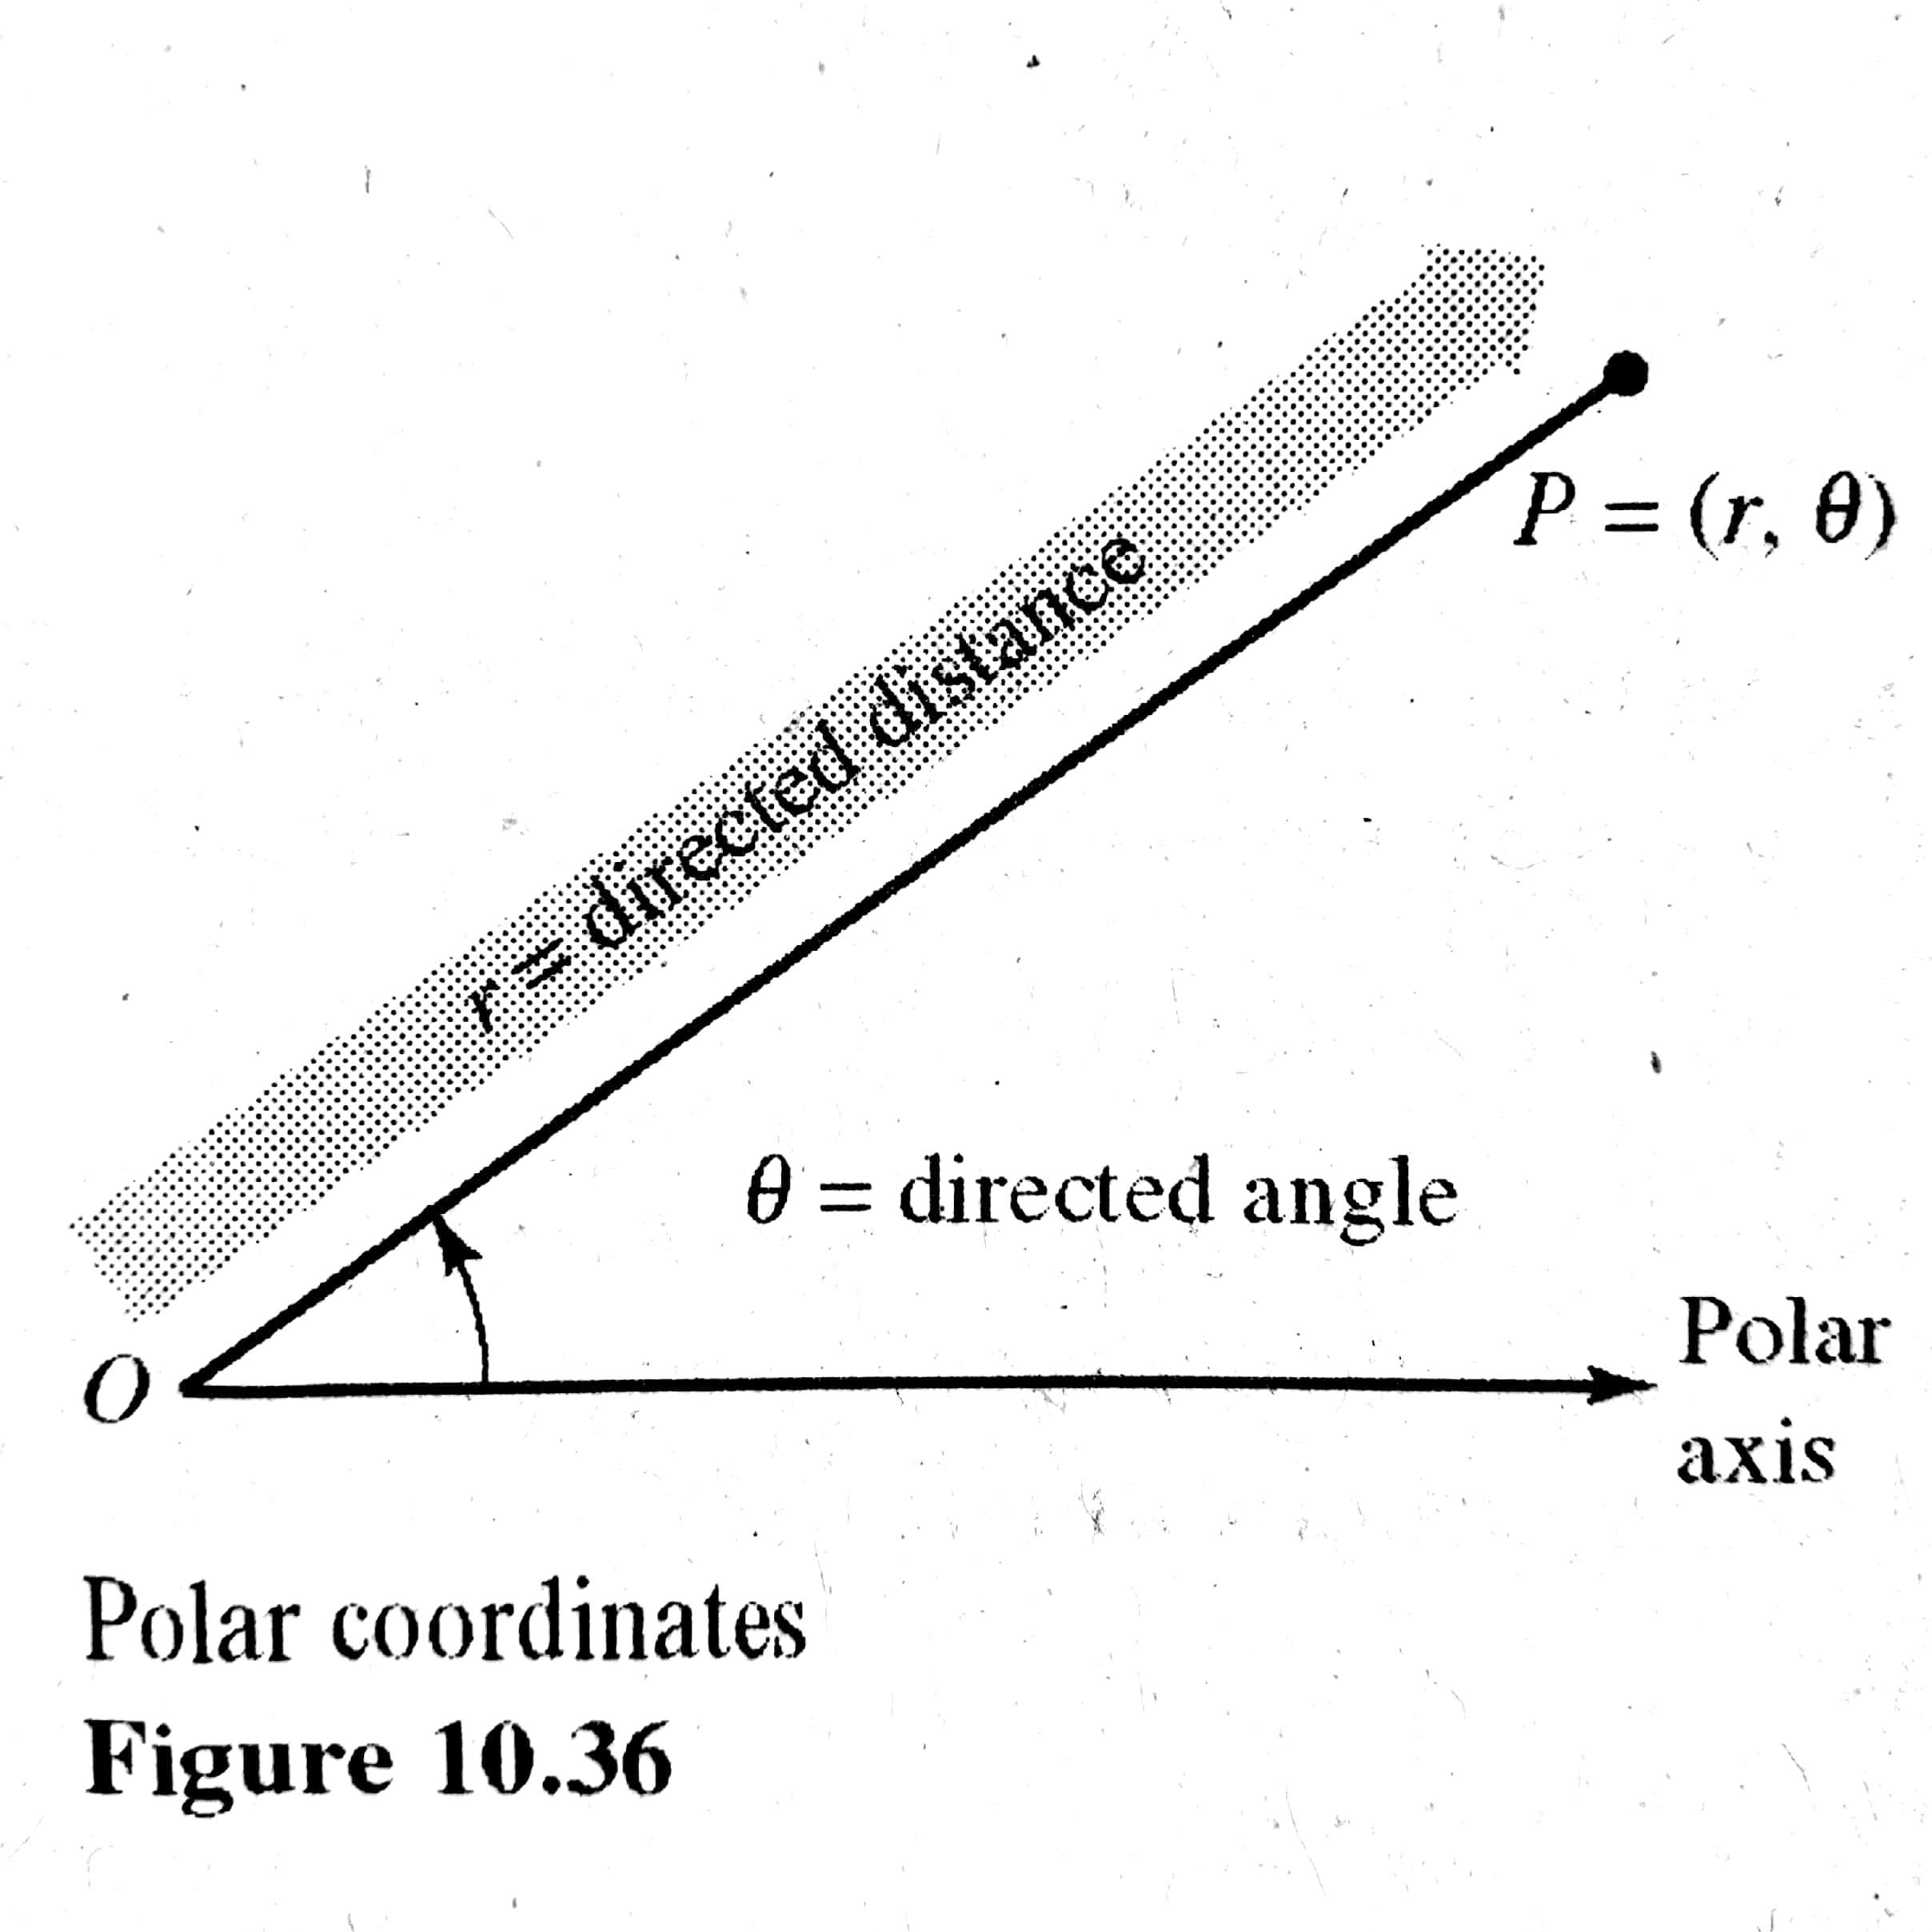
\includegraphics[height=2in]{Figure 10.36.png}
\end{figure}

\begin{enumerate}
\item r =directed distance from \emph{O} to \emph{P}
\item $\theta$ =directed angle, counterclockwise from polar axis to segment OP
\end{enumerate}

\begin{figure}[h]
\centering
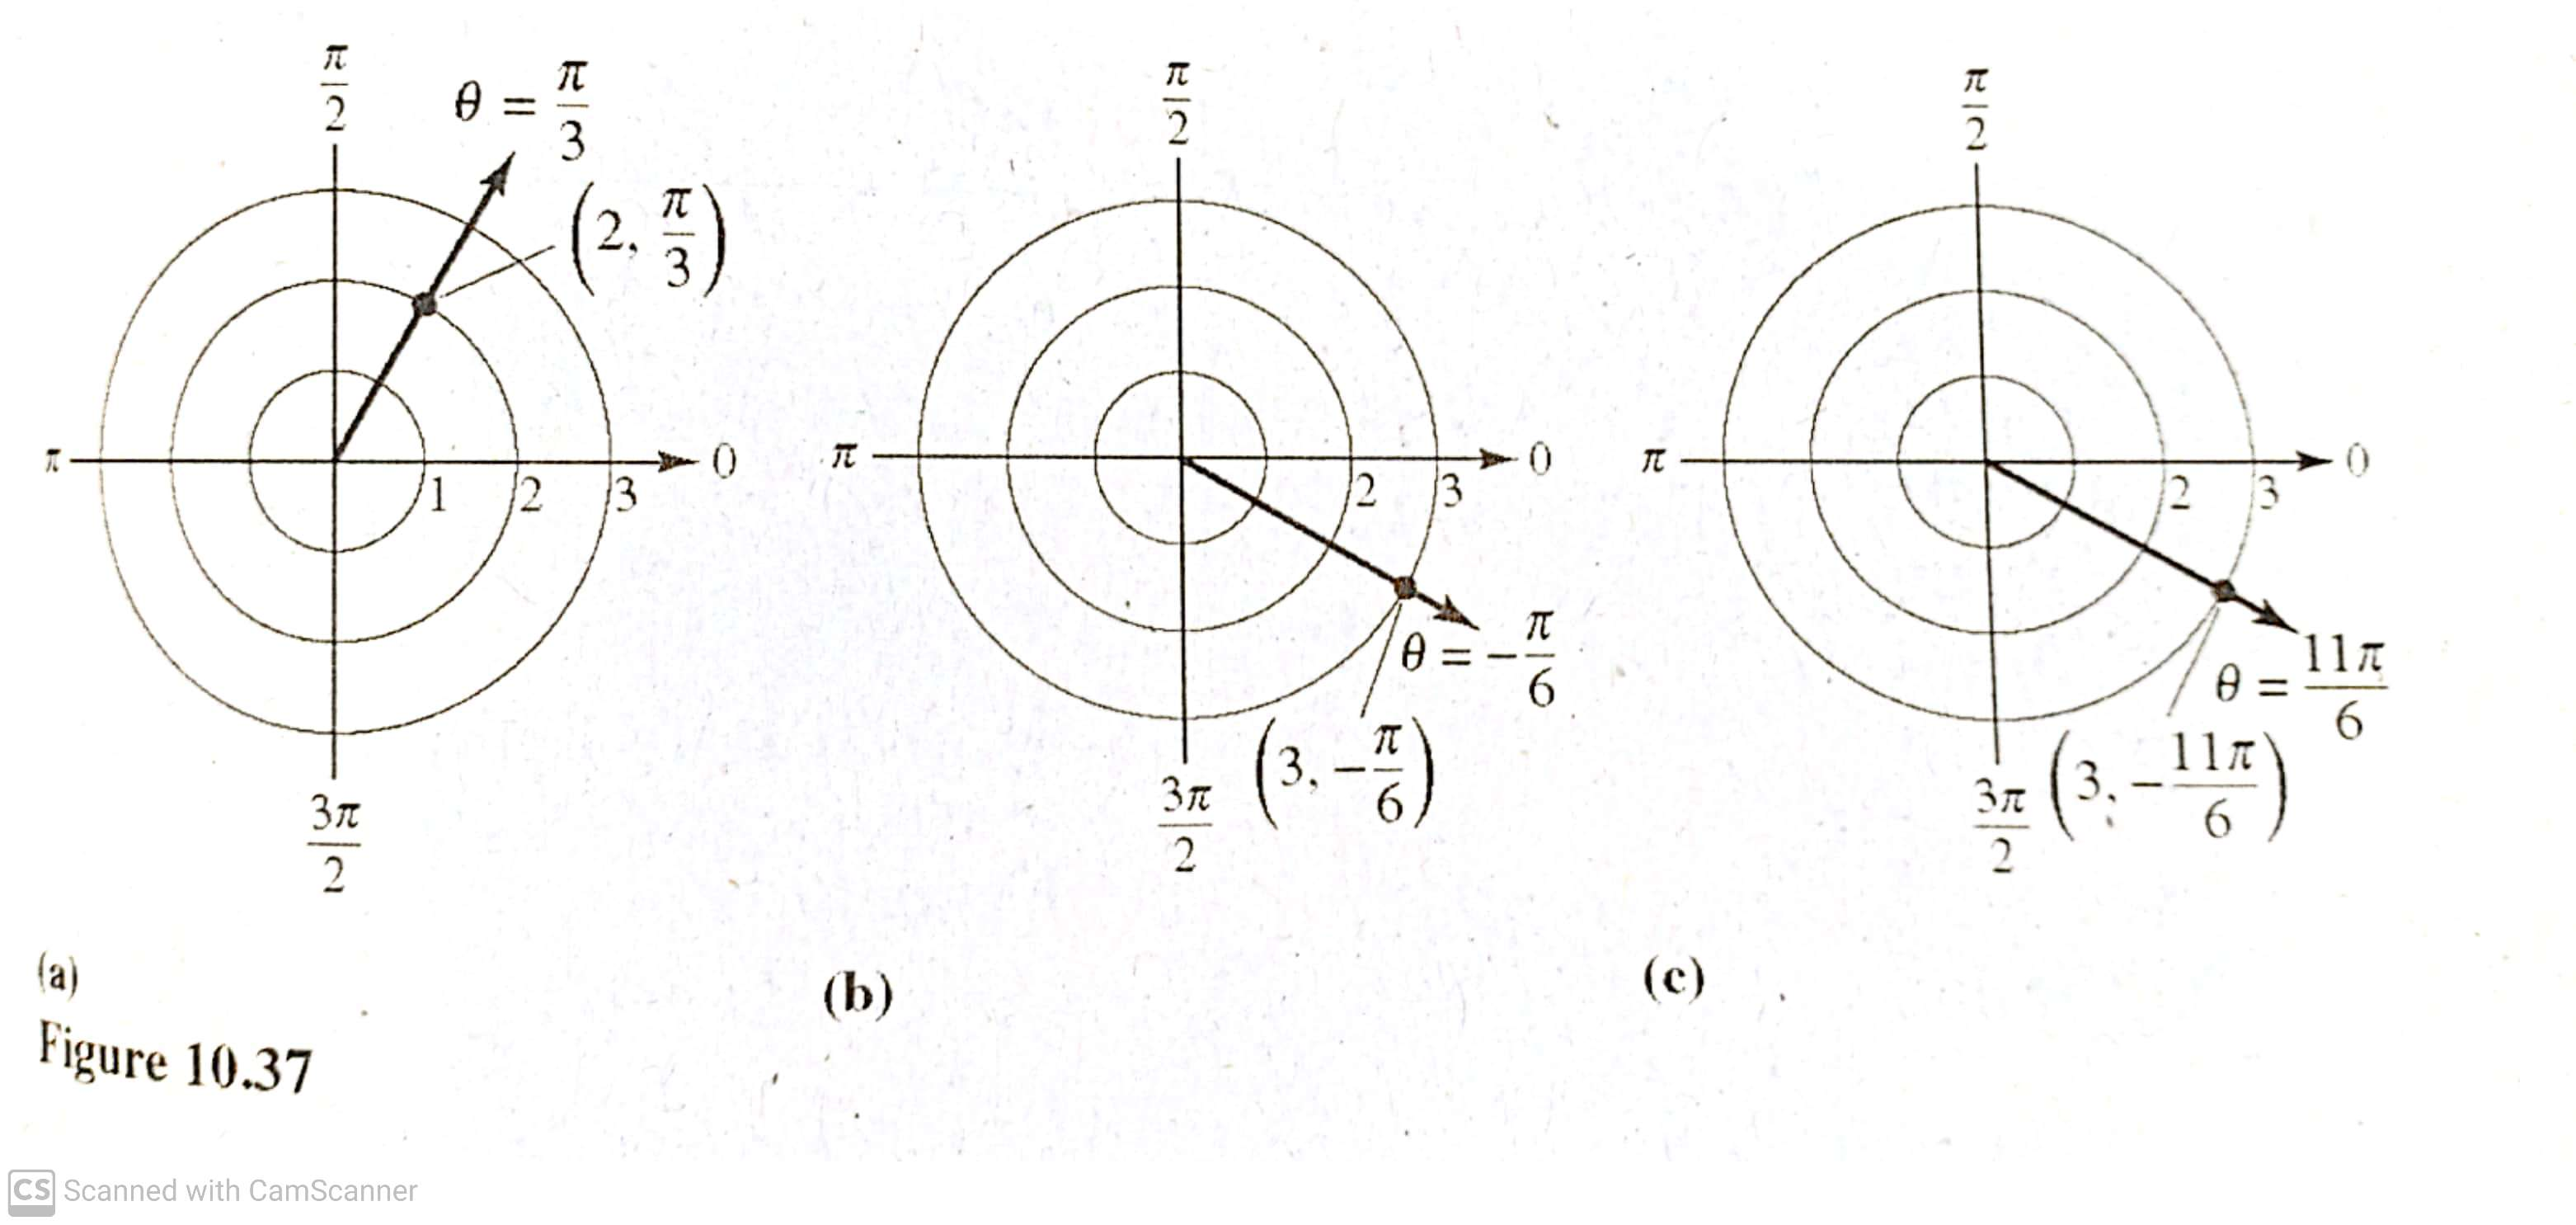
\includegraphics[height=2in]{Figure 10.37.jpg}
\end{figure}

Figure 10.37 shows three points on the polar coordinate system. Notice that in the system, it is convenient to locate points with respect to a grid of concentric circles intersected by \emph{radial line} through the pole.
With rectangular coordinates, each point \emph{(x, y)} has a unique representation. This is not true with polar coordinates.

\subsubsection{Trivia}
\textrm\emph{The mathematicians credited with first using polar coordinates was James Bernoulli, who introduced them in 1691. However, there is some evidence that it may have been Isaac Newton who first used them.}

\subsection{Coordinate Conversion}
To establish the relationship between \textbf{polar and rectangular coordinates}, let the polar axis coincide with the positive \emph{x}-axis and the pole with the origin, as shown in Figure 10.38. Because \emph{(x,y)} lies on a circle of radius \emph{r}, it follows that $r^2 = x^2 + y^2$. Moreover, for ${r}\geq 0$, the definitions of the trigonometric functions imply that
 
\begin{align*}
\sin\theta &= \frac{y}{r},\\
\cos\theta &= \frac{x}{r},\ \text{ and }\\
\tan\theta &= \frac{y}{x},
\end{align*}
if ${r}\leq 0$, you can show that the same relationships hold.

\begin{figure}[h]
\centering
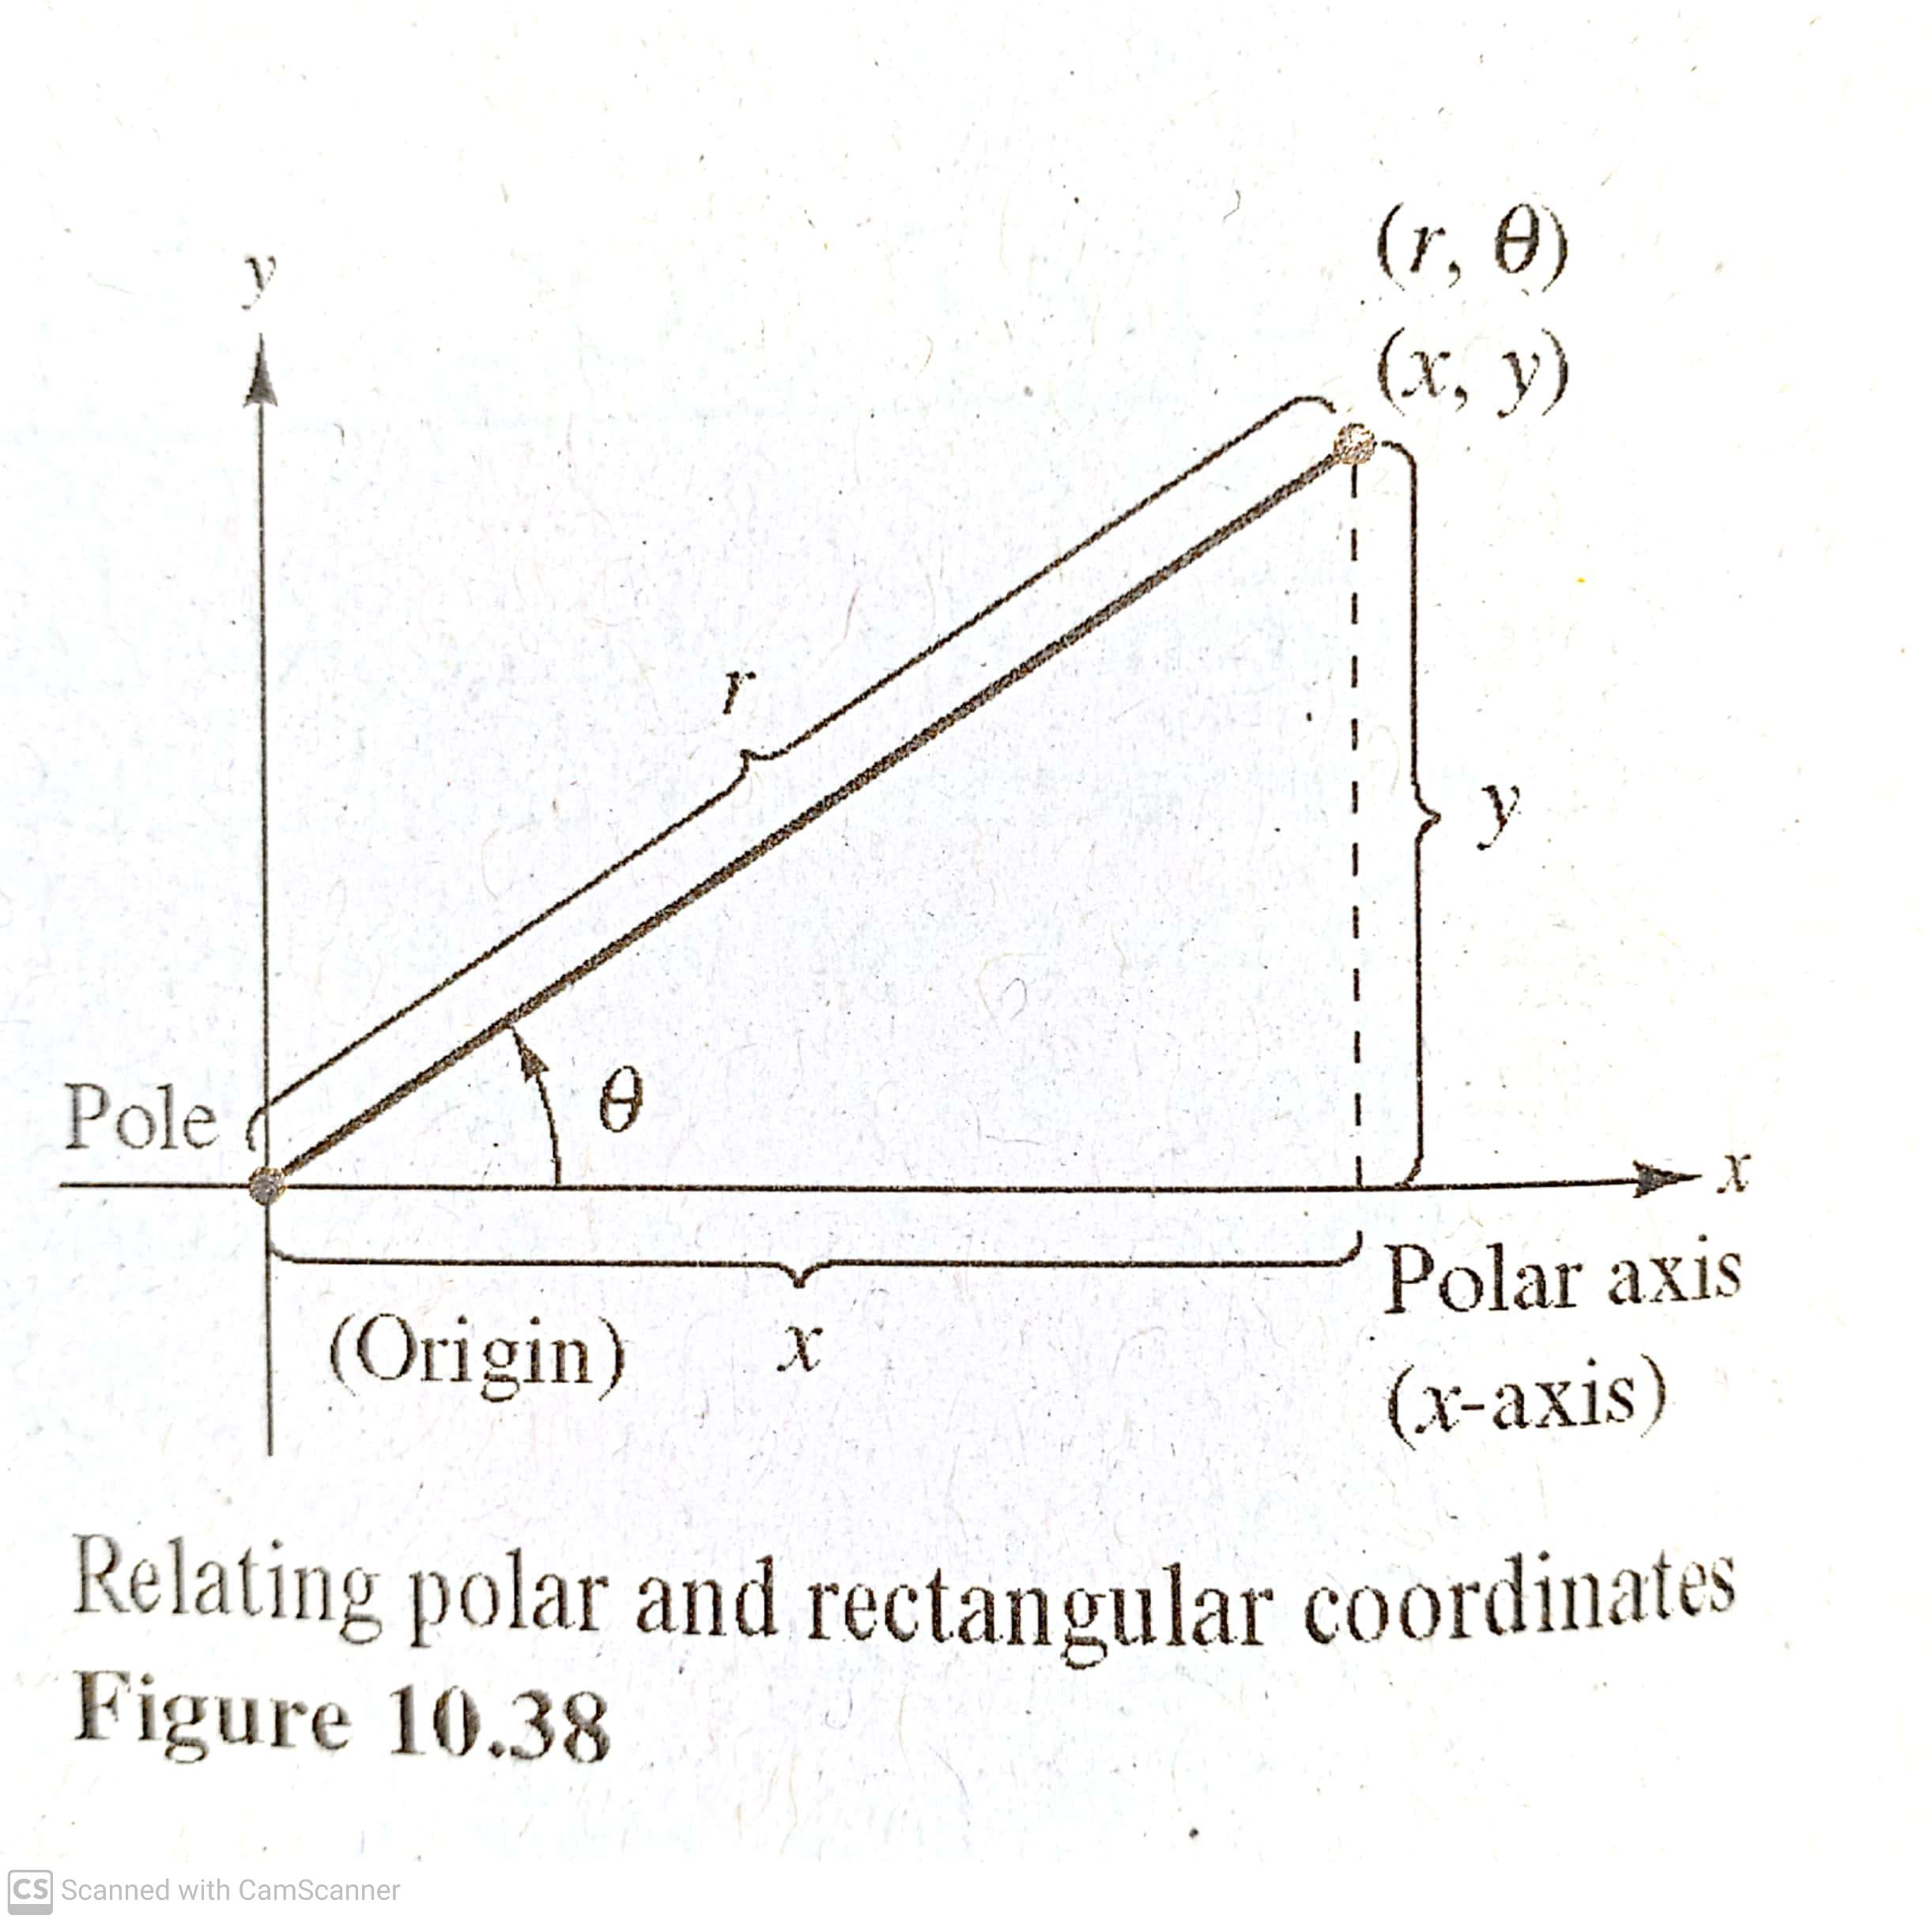
\includegraphics[height=2in]{Figure 10.38.jpg}
\end{figure}

\begin{theorem}
\textbf{COORDINATE CONVERSION} 
\\The polar coordinates $(r, \theta)$ of a point are related to the rectangular coordinates \emph{(x,y)} of the points as follows
\end{theorem}

\begin{itemize}
\item $x = r\cos\pi$     
\item $y = r\sin\pi$
\item $\tan \theta = \frac{y}{x}$
\item $r^2 = x^2 + y^2$
\end{itemize}

\begin{example}\rm
\textbf{Polar-to-Rectangular Conversion}
\\a.For the point $(r,\theta)$ = $(2,\pi)$,
$$
{x} = r\cos\theta=2\cos\pi=-2 and y=r\sin\theta=2\sin\pi=0
$$
\\So, the rectangular coordinates are (x,y)=(-2,0)
\end{example}

\begin{example}\rm
\textbf{Rectangular-to-Polar Conversion}
\\a.For the second quadrant point (x,y) = (-1,1),
$$
\tan\theta = \frac{y}{x} = -1 \Rightarrow\theta = \frac{3\pi}{4}
$$
\\Because $\theta$ was chosen to be in the same quadrant as (x,y), you should use a positive value of r.
$$
r=\sqrt{(x^2 + y^2)} = \sqrt{(-1)^2 +(1)^2} = \sqrt{2}
$$
\\This implies that \emph{one} set of Polar coordinates is $(r,\theta)$ = $(\sqrt{2},\frac{3\pi}{4})$.
\end{example}

\subsection{Polar Graphs}
One way to sketch the graph of a polar equation is to convert to rectangular coordinates and then sketch the graph of the rectangular equation.

\begin{example}\rm
\textbf{Graphing Polar Equations}
\\Describe the graph of each polar equation. Confirm each description by converting to a rectangular equation.
\\\\a.r=$\sec\theta$
\\The graph of the polar equation r=$\sec\theta$ is not evident by simple inspection, so you can begin by converting to rectangular form using the relationship r = $\cos\theta$ = x
$$
\\r=\sec\theta
\\r\cos\theta=1
\\x=1
$$
\\ b.$\theta=\frac{\pi}{3}$
\\The graph of the polar equation $\theta=\frac{\pi}{3}$ consists  of all points on the line that makes an angle of $\frac{\pi}{3}$ woth the positive x-axis. You can confirm this by using the relationship $\tan\pi = \frac{y}{x}$ to obtain the rectangular equation
$$
y=\sqrt{3}x
$$
\end{example}

\begin{thebibliography}{2}
\bibitem{ll} {\bf Larson \& Edwards}, Calculus.
\end{thebibliography}
\end{document}